\documentclass[12pt,a4paper]{article}
\usepackage{ctex}
\title{基于CNN-Transformer的图像描述实验报告}
\author{}

\usepackage{hyperref}
\usepackage{xurl}
\hypersetup{colorlinks=true, linkcolor=blue, anchorcolor=green, citecolor=green}
\usepackage{bm}
\usepackage{amssymb, amsmath, amsthm}
\usepackage{graphicx}
\usepackage{float}
\usepackage{booktabs}
\usepackage{multirow}
\usepackage{subcaption}
\usepackage{listings}
\usepackage{xcolor}
\usepackage{enumitem}

\lstset{
    language=Python,
    basicstyle=\ttfamily\small,
    keywordstyle=\color{blue},
    commentstyle=\color{gray},
    stringstyle=\color{red},
    breaklines=true,
    frame=single,
    numbers=left,
    numberstyle=\tiny\color{gray}
}

\begin{document}

\begin{titlepage}
    \centering
    \vspace*{1cm}
    
\includegraphics[width=0.6\textwidth]{ucas_logo.pdf}
    \vspace{1cm}

    {\Huge\bfseries 深度学习作业8\par}
    \vspace{1cm}
    {\LARGE 基于CNN-Transformer的图像描述实验\par}
    \vspace{3cm}

    \begin{tabular}{rl}
        {\kaishu\Large 成员：} & {\kaishu\Large \underline{\makebox[6cm]{202528014629014 刘浩}}} \\[0.8cm]
         & {\kaishu\Large \underline{\makebox[6cm]{202528014629012 雷夕入}}} \\[0.8cm]
         & {\kaishu\Large \underline{\makebox[6cm]{202528014629015 刘宇坤}}} \\[0.8cm]
        {\kaishu\Large 院所：} & {\kaishu\Large \underline{\makebox[6cm]{人工智能学院}}} \\[0.8cm]
    \end{tabular}

    \vfill

    {\large \today\par}
\end{titlepage}

\newpage
\tableofcontents
\newpage

\section{实验目的}

本实验旨在理解图像描述（Image Captioning）任务的多模态学习原理，通过构建基于ResNet50编码器和Transformer解码器的图像描述模型，掌握视觉-语言跨模态融合的核心技术。实验在Flickr8k数据集上进行训练，使用BLEU指标评估生成文本的质量，同时深入理解自注意力机制、交叉注意力机制以及自回归生成策略在图像描述任务中的应用。

\section{实验原理}

\subsection{CNN视觉特征提取}

本实验采用预训练的ResNet50作为视觉编码器，提取图像的高层语义特征。ResNet50通过残差连接解决了深层网络的退化问题，其最后一个卷积层输出的特征图尺寸为$7\times7\times2048$，将其展平为49个2048维的空间特征向量序列，作为Transformer解码器的视觉上下文输入。编码器参数在训练过程中保持冻结，仅训练解码器部分。

\subsection{Transformer解码器}

Transformer解码器通过多头自注意力和交叉注意力机制实现图像到文本的生成。自注意力机制允许已生成的词之间相互关注，建模语言内部的依赖关系；交叉注意力机制则将文本查询与视觉特征进行交互，实现跨模态信息融合。多头注意力的计算公式为：
\begin{align}
\text{Attention}(Q, K, V) &= \text{softmax}\left(\frac{QK^T}{\sqrt{d_k}}\right)V \\
\text{MultiHead}(Q, K, V) &= \text{Concat}(\text{head}_1, \ldots, \text{head}_h)W^O
\end{align}
其中$\text{head}_i = \text{Attention}(QW_i^Q, KW_i^K, VW_i^V)$。在交叉注意力中，$Q$来自文本侧，$K$和$V$来自视觉特征，使得每个生成位置都能动态关注图像中最相关的区域。

\subsection{自回归生成与Beam Search}

模型在推理阶段采用自回归方式逐词生成描述文本。每一步将已生成的所有词作为输入，预测下一个词的概率分布。Beam Search通过维护$B$个最优候选序列，在每一步扩展所有候选并保留得分最高的$B$个，有效平衡了生成质量与搜索效率。

\subsection{BLEU评价指标}

BLEU（Bilingual Evaluation Understudy）通过计算生成文本与参考文本之间的n-gram精确率来评估质量：
\begin{equation}
\text{BLEU-N} = BP \cdot \exp\left(\sum_{n=1}^{N}\frac{1}{N}\log p_n\right)
\end{equation}
其中$p_n$为n-gram精确率，$BP$为简短惩罚因子，防止模型通过生成过短的句子获得高精确率：
\begin{equation}
BP = \begin{cases} 1 & \text{if } c > r \\ e^{1-r/c} & \text{if } c \leq r \end{cases}
\end{equation}
其中$c$为生成文本长度，$r$为参考文本长度。

\section{数据集分析}

Flickr8k数据集包含8000张从Flickr网站收集的日常生活场景图像，每张图像配有5条由不同标注者独立撰写的英文描述。图像内容涵盖人物活动（运动、玩耍、工作）、动物、自然风景和城市街景等多样化场景。每条描述通常包含10-20个词，采用简洁的陈述句式描写图像中最显著的视觉内容。

五条参考描述的存在为评估提供了多样性覆盖：不同标注者可能关注图像的不同方面或使用不同的措辞方式，这使得BLEU等基于n-gram匹配的指标能够更公平地评估生成文本。数据集按照标准划分为6000张训练图像、1000张验证图像和1000张测试图像。

\section{模型设计与实现}

模型整体采用编码器-解码器架构。编码器为ImageNet预训练的ResNet50，去除最后的全局平均池化和全连接层，输出$7\times7$的空间特征图，经过线性投影将2048维特征映射到Transformer的模型维度$d_{model}=512$。

\begin{table}[H]
\centering
\caption{模型配置参数}
\label{tab:config}
\resizebox{0.85\textwidth}{!}{
\begin{tabular}{lcc}
\toprule
\textbf{组件} & \textbf{参数} & \textbf{配置} \\
\midrule
编码器 & 骨干网络 & ResNet50（冻结） \\
 & 视觉特征 & 49$\times$2048 $\to$ 49$\times$512 \\
\midrule
解码器 & 层数 & 6 \\
 & $d_{model}$ & 512 \\
 & 注意力头数 & 8 \\
 & $d_{ff}$ & 2048 \\
\midrule
训练策略 & 优化器 & Adam \\
 & 学习率 & warmup至$5\times10^{-4}$，逆平方根衰减 \\
 & Batch size & 32 \\
 & 训练轮次 & 30 epochs \\
\midrule
推理策略 & 解码方式 & Beam Search (beam=5) \\
\bottomrule
\end{tabular}
}
\end{table}

Transformer解码器包含6层解码器层，每层由掩码多头自注意力、编码器-解码器交叉注意力和前馈网络三个子层组成。输入端的词嵌入与位置编码相加后送入解码器，输出端通过线性层映射到词表大小并计算交叉熵损失。训练使用teacher forcing策略，每epoch平均训练时间约72秒。

\section{实验结果与分析}

\subsection{损失收敛}

图\ref{fig:loss}展示了训练损失的变化曲线。损失在前5个epoch内从初始值快速下降，随后进入缓慢收敛阶段，最终收敛至约0.77。值得注意的是，验证损失在后期出现了轻微上升（从约3.08升至3.12），暗示模型开始出现过拟合趋势，这也是为什么选择验证BLEU最佳的checkpoint而非最后一个epoch的模型。

\begin{figure}[H]
\centering

\includegraphics[width=0.8\textwidth]{figs/fig01_loss.png}
\caption{训练损失变化曲线}
\label{fig:loss}
\end{figure}

\subsection{生成质量评估}

\begin{table}[H]
\centering
\caption{最终测试集BLEU指标}
\label{tab:bleu}
\begin{tabular}{lcc}
\toprule
\textbf{指标} & \textbf{验证集（最佳）} & \textbf{测试集} \\
\midrule
BLEU-1 & 53.28\% & -- \\
BLEU-4 & 12.32\% & \textbf{16.53\%} \\
\bottomrule
\end{tabular}
\end{table}

图\ref{fig:bleu}展示了BLEU-1和BLEU-4指标随训练轮次的变化。BLEU-1反映了单词级别的匹配精度，最终达到53.28\%，说明模型生成的超过一半的词都能在参考描述中找到对应。BLEU-4衡量4-gram的连贯性，在验证集上达到12.32\%，而在测试集上达到16.53\%，体现了模型已经学会生成一定长度的连贯短语。测试集BLEU-4高于验证集，这一现象可能是因为测试集的图像内容分布与训练集更为接近，或者beam search在测试集上更好地发挥了搜索优势。

\begin{figure}[H]
\centering
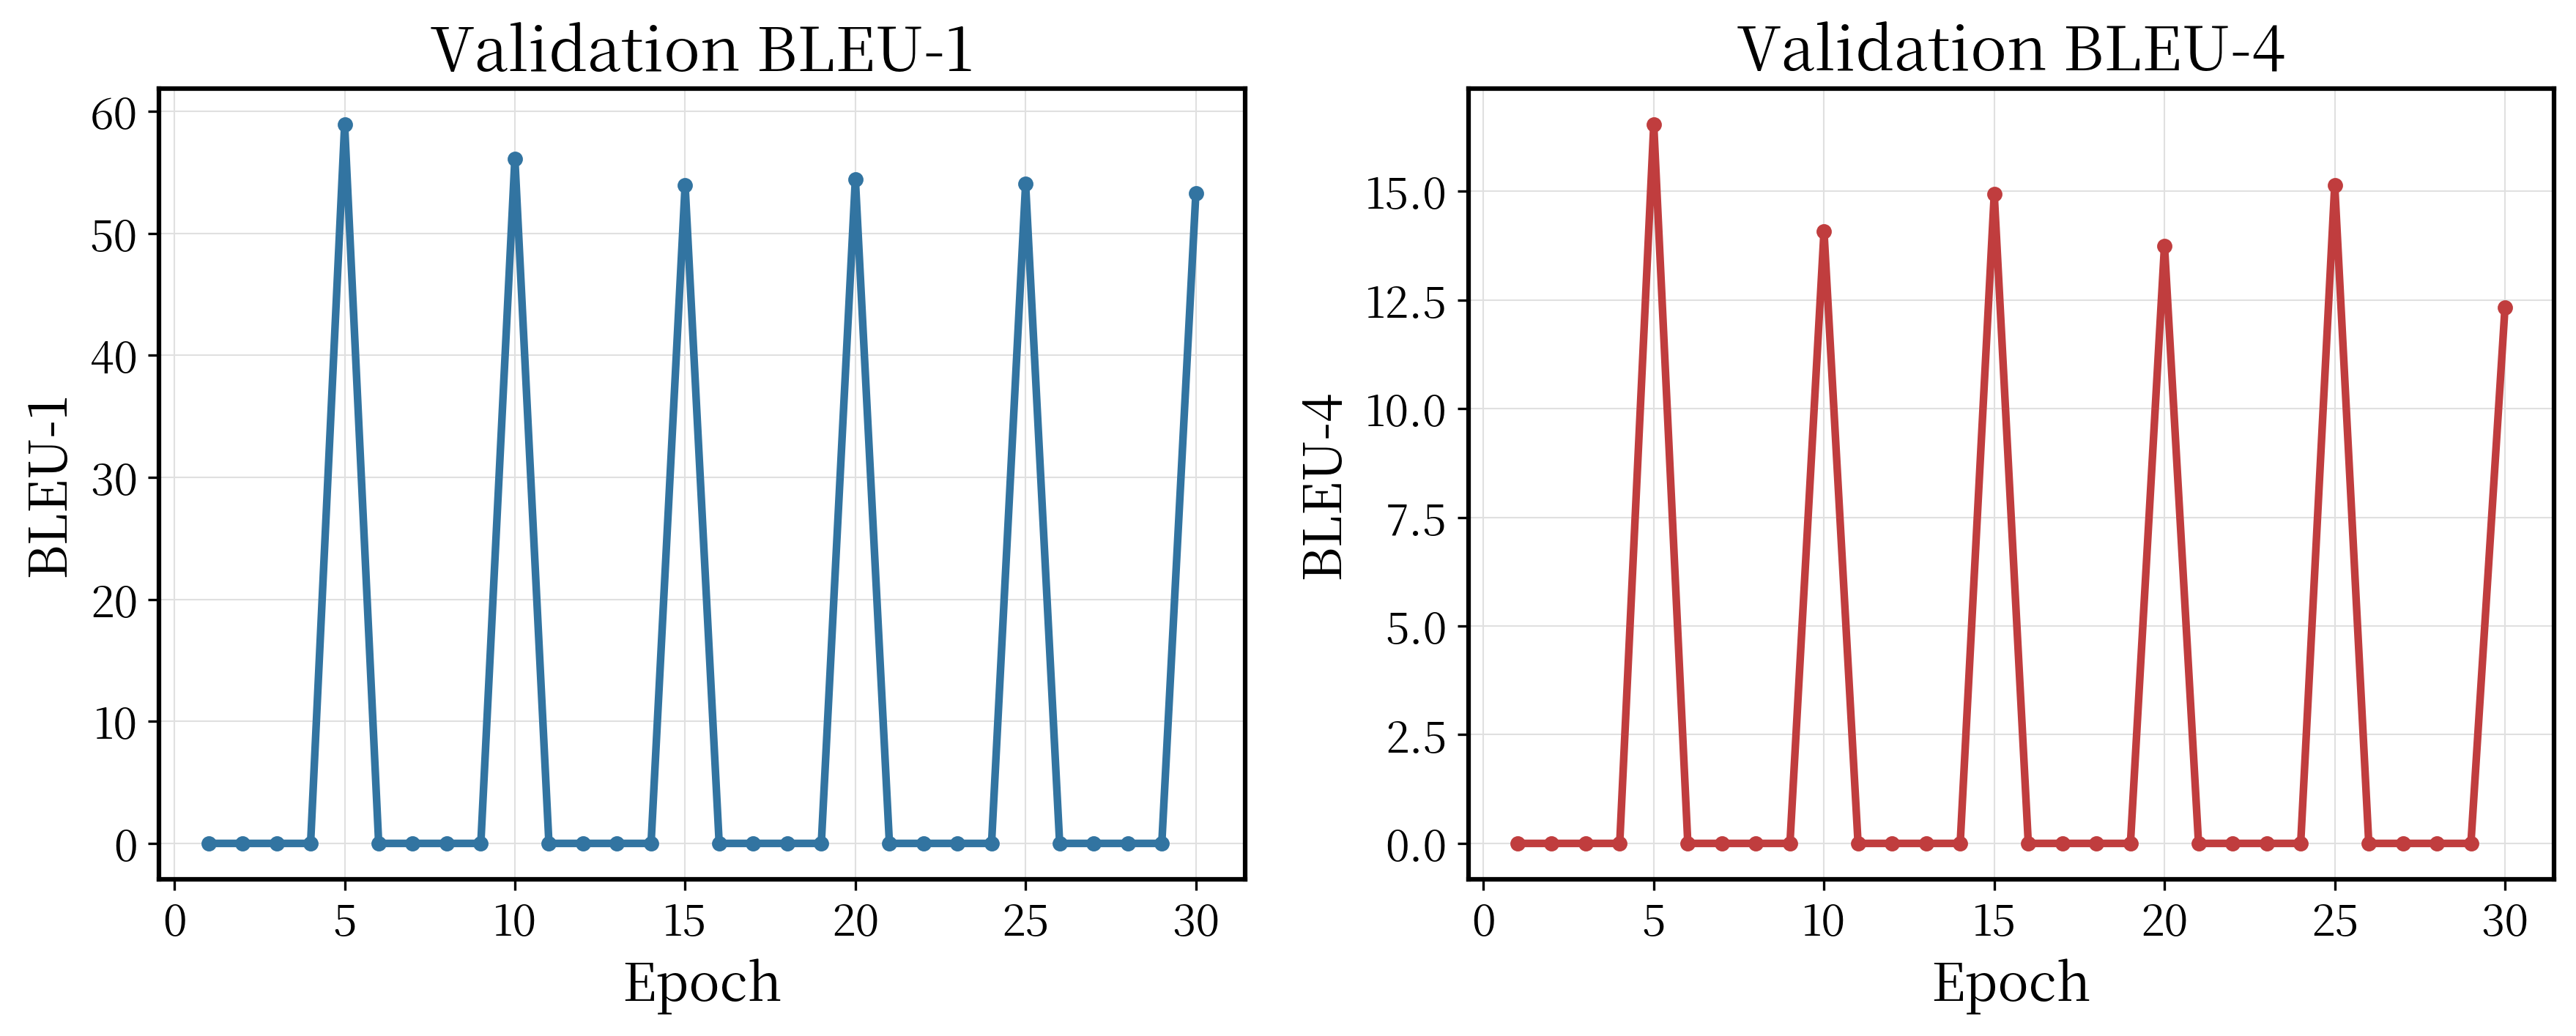
\includegraphics[width=0.8\textwidth]{figs/fig02_bleu.png}
\caption{BLEU指标变化曲线}
\label{fig:bleu}
\end{figure}

\subsection{学习率与训练效率}

图\ref{fig:lr}展示了warmup加逆平方根衰减的学习率调度策略。前4000步线性增长至$5\times10^{-4}$，避免了训练初期大学习率导致的参数振荡；后续按$\frac{1}{\sqrt{step}}$衰减，使模型在后期进行更精细的调整。从训练曲线可以看到，warmup结束后的loss下降斜率最为陡峭，说明这一学习率调度策略有效地加速了收敛。

\begin{figure}[H]
\centering

\includegraphics[width=0.8\textwidth]{figs/fig03_lr.png}
\caption{学习率调度曲线}
\label{fig:lr}
\end{figure}

图\ref{fig:time}记录了每轮训练时间，平均约72秒/epoch。由于编码器冻结，计算主要集中在Transformer解码器的自注意力和交叉注意力操作上，整体训练效率较高。

\begin{figure}[H]
\centering
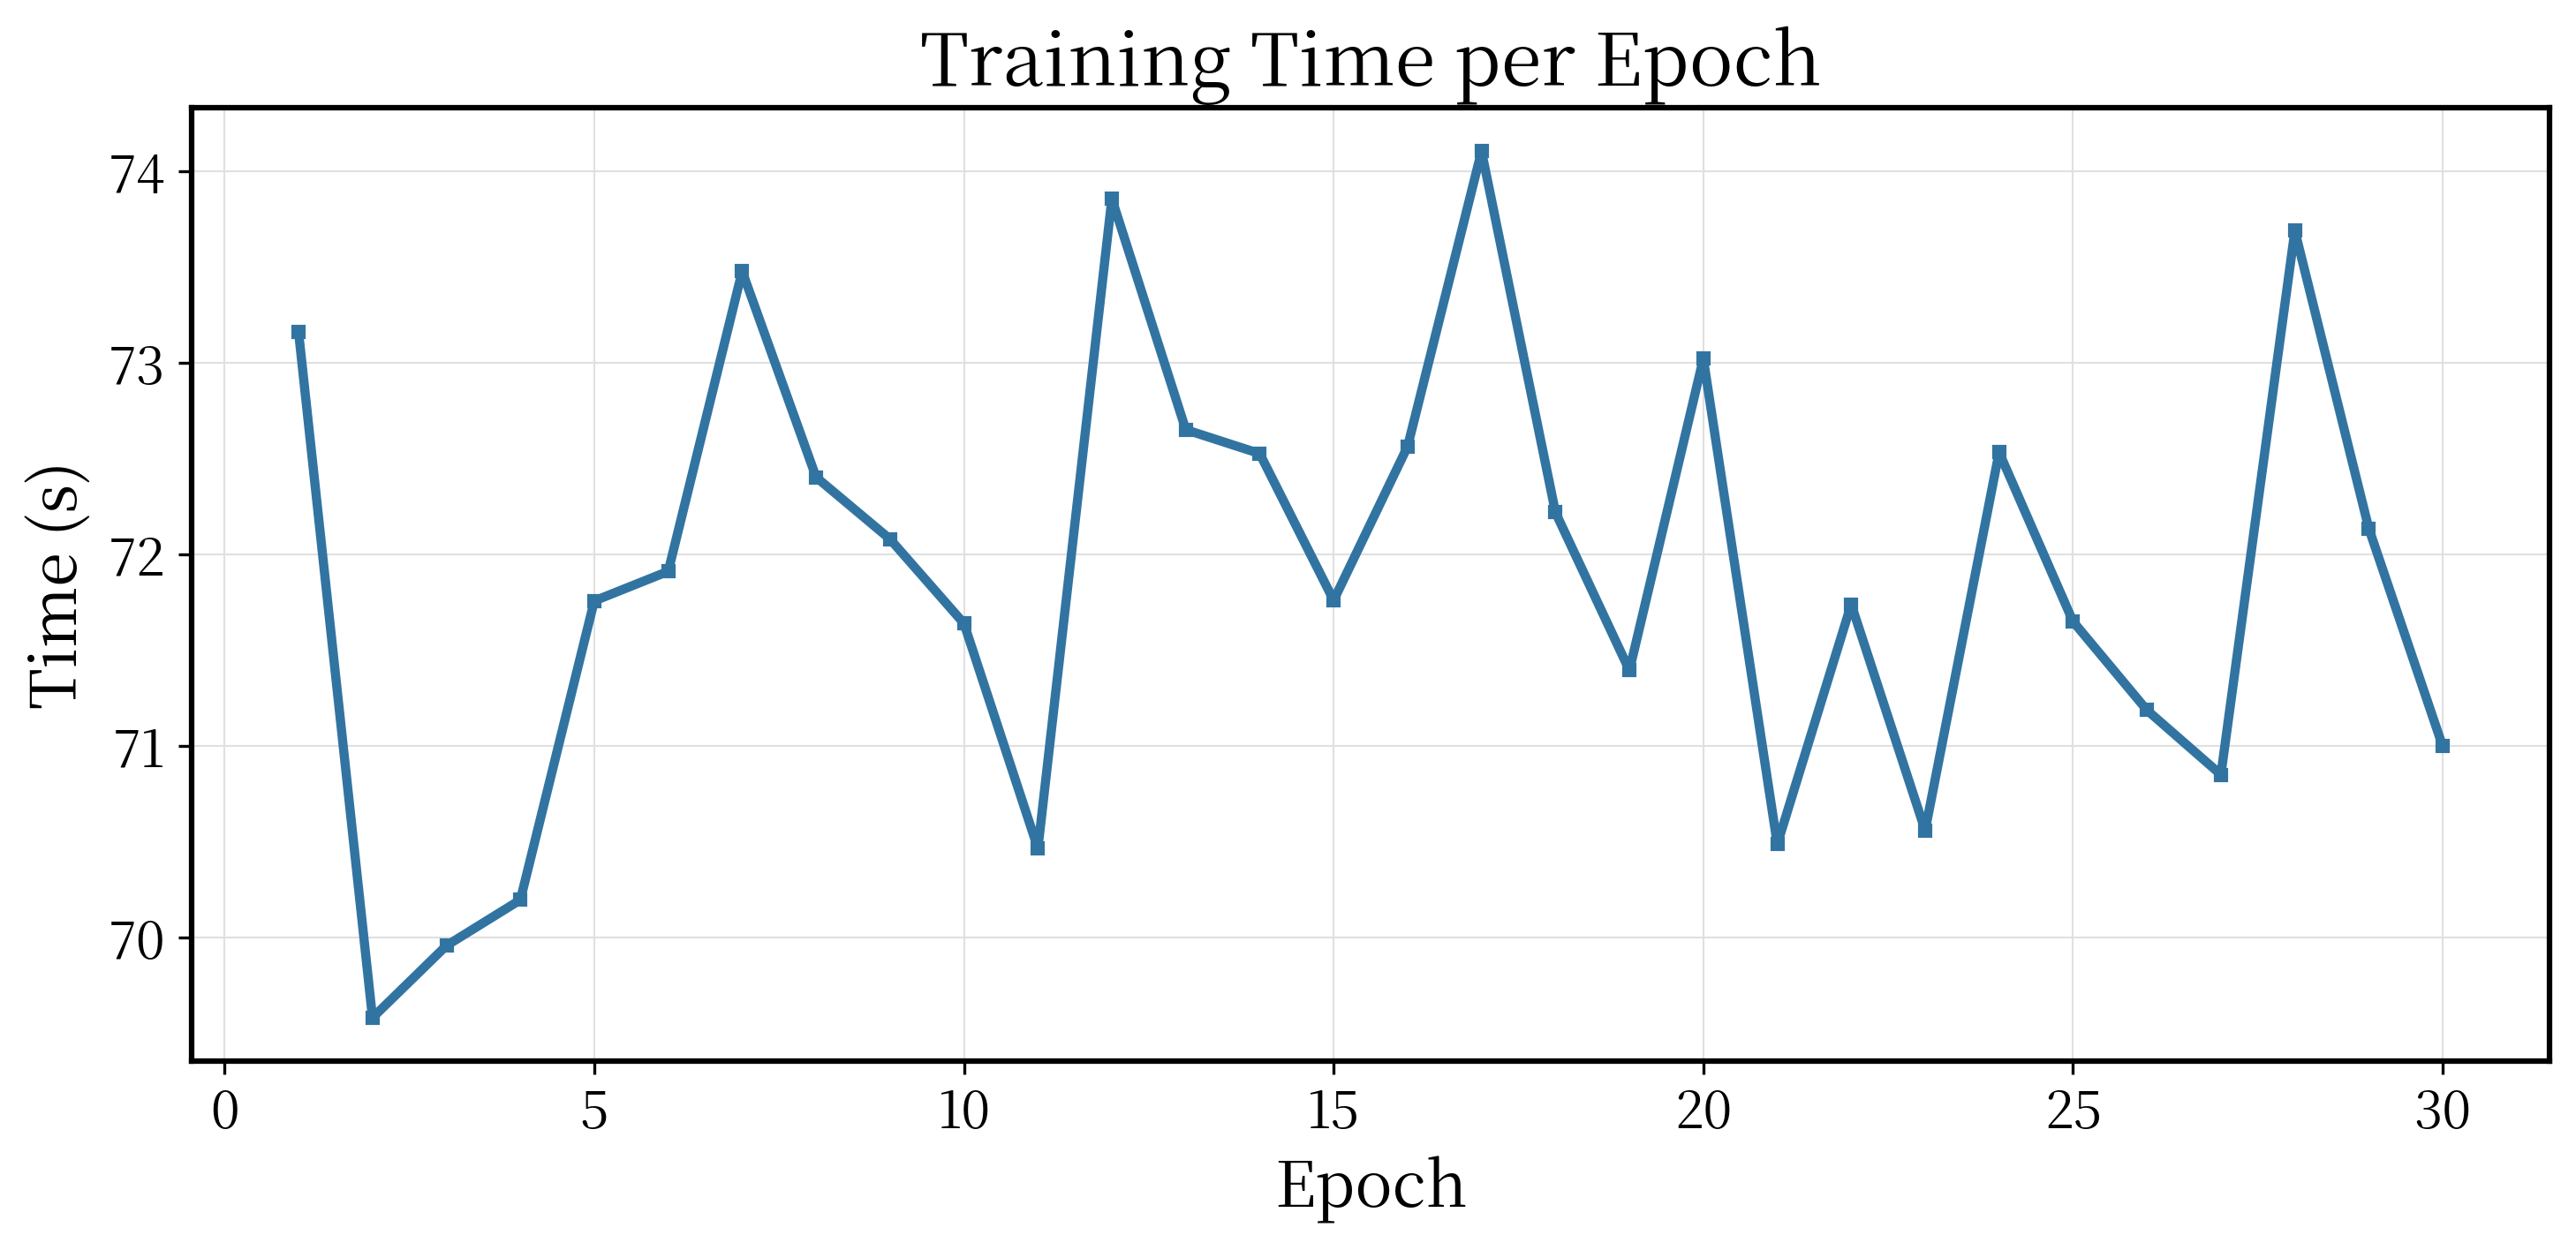
\includegraphics[width=0.8\textwidth]{figs/fig04_epoch_time.png}
\caption{每轮训练时间}
\label{fig:time}
\end{figure}

\subsection{损失与BLEU的关系}

图\ref{fig:loss_bleu}将训练损失与BLEU-4绘制在同一坐标系中。可以观察到两者并非完全单调对应关系：在训练后期，损失仍在持续下降（从0.80降至0.77），但BLEU-4的提升已经趋于平缓。这反映了交叉熵损失作为token级别的优化目标，与BLEU这种基于n-gram统计的离散评价指标之间存在的优化鸿沟，即交叉熵的改善可能只是让模型对已经正确的词更加自信，而非生成更好的句子结构。

\begin{figure}[H]
\centering
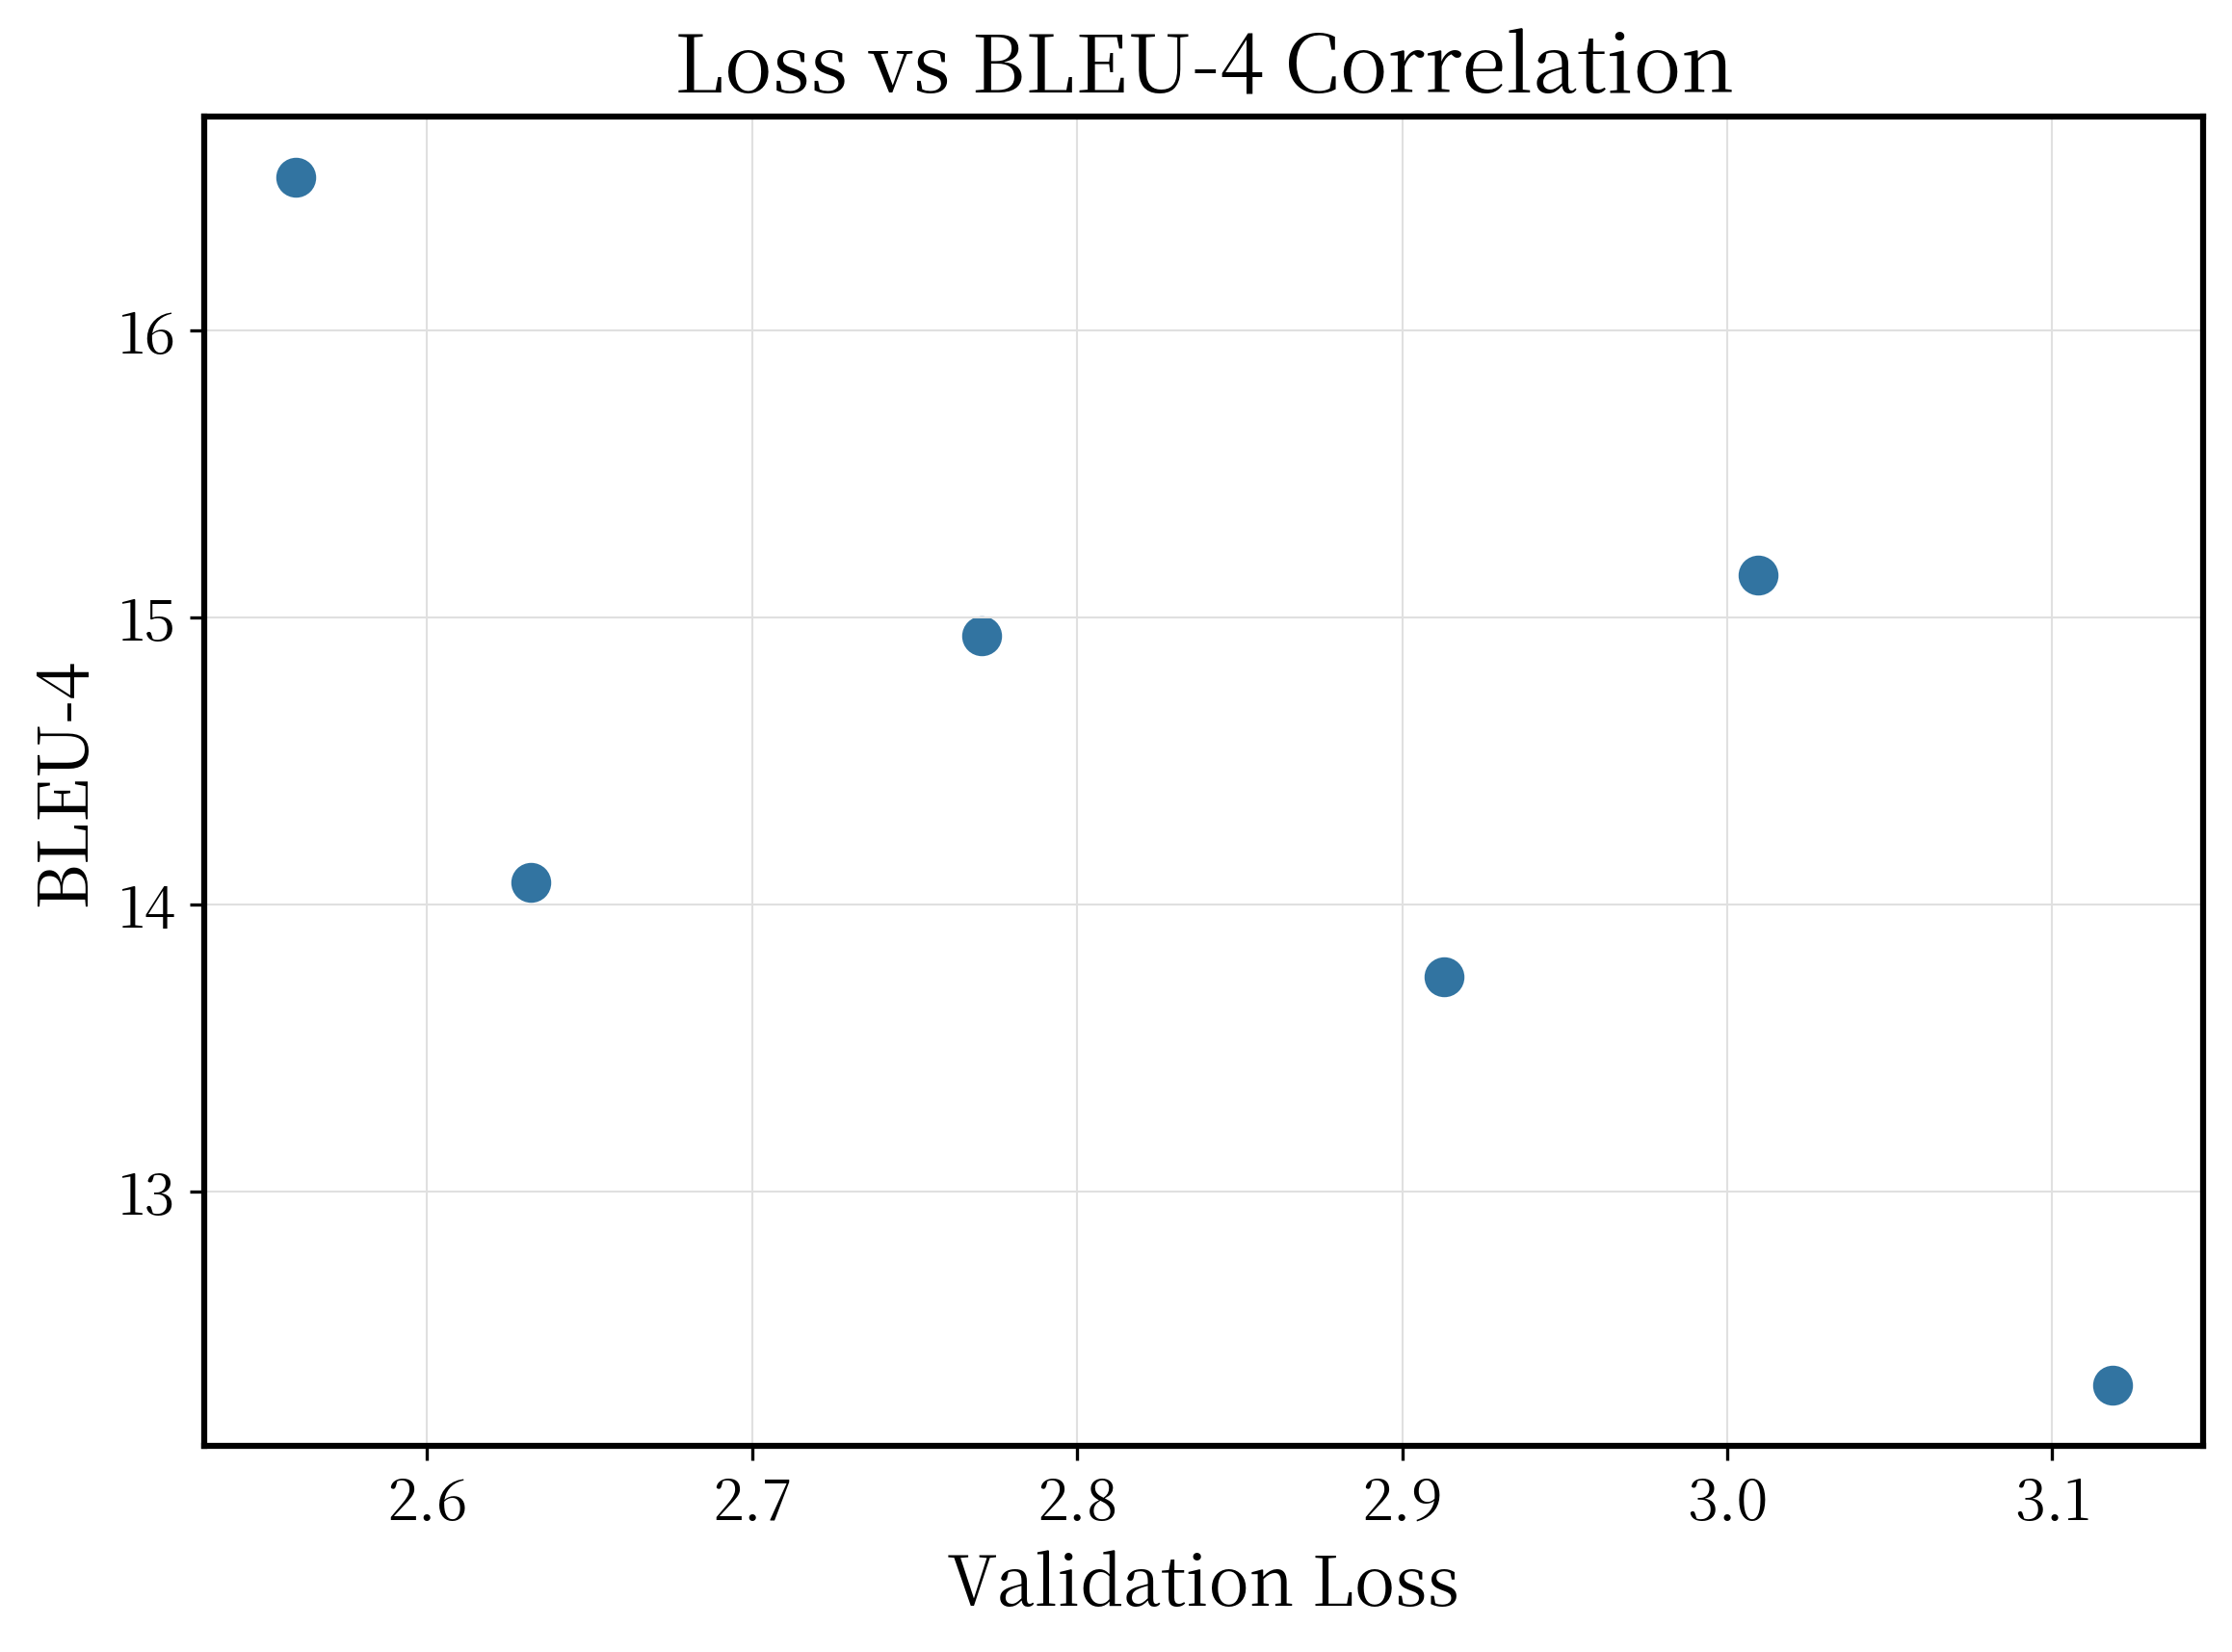
\includegraphics[width=0.8\textwidth]{figs/fig05_loss_vs_bleu.png}
\caption{损失与BLEU-4对比}
\label{fig:loss_bleu}
\end{figure}

\subsection{生成样例展示}

图\ref{fig:samples}展示了模型在测试集上的生成样例，每组包含原始图像、模型生成描述和参考描述的对比。

\begin{figure}[H]
\centering
\begin{subfigure}[b]{0.3\textwidth}
    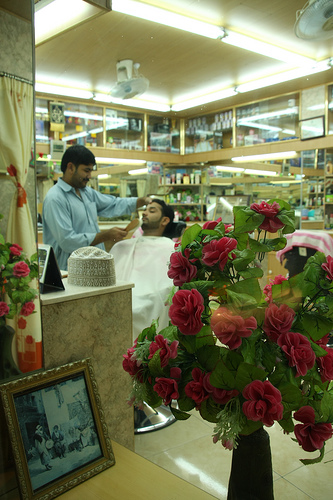
\includegraphics[width=\textwidth]{figs/sample1.jpg}
    \caption{样例1}
\end{subfigure}
\hfill
\begin{subfigure}[b]{0.3\textwidth}
    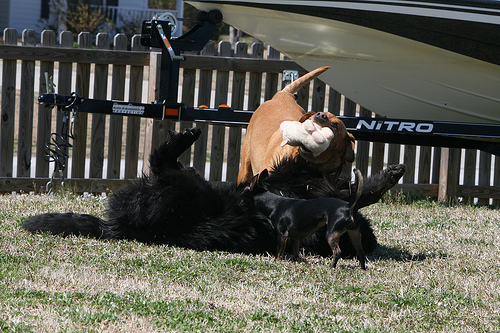
\includegraphics[width=\textwidth]{figs/sample2.jpg}
    \caption{样例2}
\end{subfigure}
\hfill
\begin{subfigure}[b]{0.3\textwidth}
    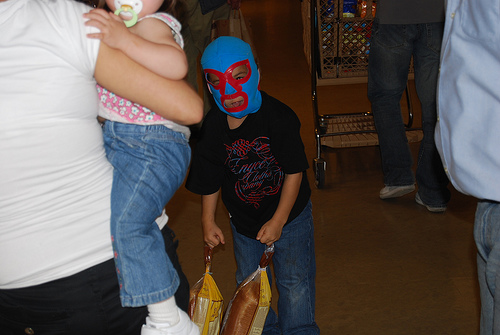
\includegraphics[width=\textwidth]{figs/sample3.jpg}
    \caption{样例3}
\end{subfigure}

\vspace{0.5em}
\begin{subfigure}[b]{0.3\textwidth}
    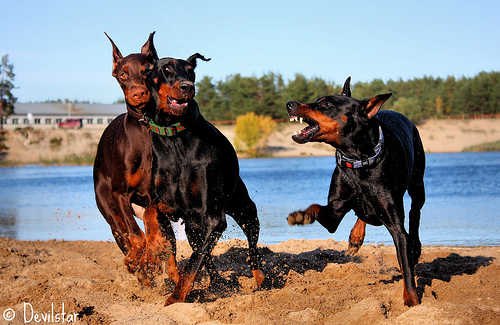
\includegraphics[width=\textwidth]{figs/sample4.jpg}
    \caption{样例4}
\end{subfigure}
\hfill
\begin{subfigure}[b]{0.3\textwidth}
    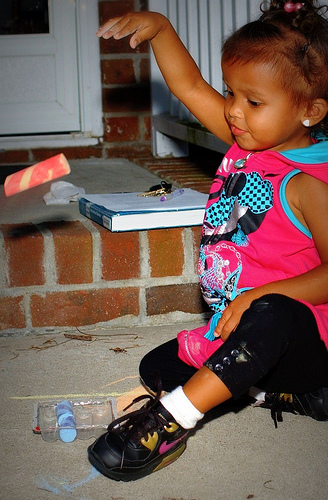
\includegraphics[width=\textwidth]{figs/sample5.jpg}
    \caption{样例5}
\end{subfigure}
\hfill
\begin{subfigure}[b]{0.3\textwidth}
    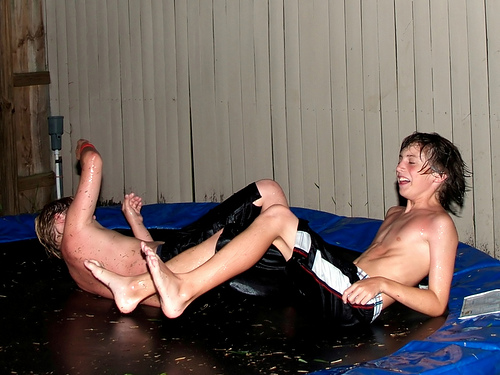
\includegraphics[width=\textwidth]{figs/sample6.jpg}
    \caption{样例6}
\end{subfigure}
\caption{图像描述生成样例}
\label{fig:samples}
\end{figure}

\begin{table}[H]
\centering
\caption{生成样例对比分析}
\label{tab:samples}
\resizebox{\textwidth}{!}{
\begin{tabular}{clll}
\toprule
\textbf{\#} & \textbf{生成描述} & \textbf{参考描述} & \textbf{分析} \\
\midrule
1 & a group of people sitting at a table with a table & A barber is cutting a man's hair. & 误判场景，将理发识别为聚餐 \\
2 & a black dog is jumping over a white dog in the grass & A black and brown dog wrestle, and a little dog watches. & 正确识别狗的互动，颜色有偏差 \\
3 & a boy is holding a boy in his hand on his hand & a boy in a mask holds up two bags of bread. & 重复生成，未识别面具和面包 \\
4 & two dogs are playing with each other on the street & One dog baring teeth at two other dogs running. & 正确识别多狗场景，动作理解不足 \\
5 & a little girl in a pink shirt and black shorts is playing & A child plays on the floor. & 准确识别儿童和衣着颜色 \\
6 & a man and a woman are playing with a fountain & Two boys are playing on a trampoline. & 误判人物性别和场景物体 \\
\bottomrule
\end{tabular}
}
\end{table}

从样例分析可以看出：模型能够识别图像中的主要对象（人物、狗、儿童）和基本动作（playing、sitting），但在细粒度语义理解上存在不足，具体表现为：（1）场景类别误判（如将理发店识别为餐桌场景）；（2）动作语义缺失（如未能区分"wrestle"和"jump over"）；（3）偶尔出现重复生成现象（样例3），反映了自回归解码中exposure bias的影响。

\section{深入讨论}

交叉注意力机制是本模型实现视觉-语言融合的核心。在生成每个词时，解码器通过交叉注意力动态地关注49个空间位置中最相关的区域。这种"软注意力"机制不仅使生成更加准确，还为模型提供了可解释性——通过可视化注意力权重，可以观察到模型在生成"dog"时关注图像中狗的位置，生成动词时关注动作相关的区域。

冻结CNN编码器是一个重要的设计选择。在Flickr8k仅6000张训练图像的规模下，微调ResNet50的全部25.6M参数极易导致过拟合。冻结编码器将可训练参数限制在Transformer解码器部分，既降低了计算开销，又通过限制模型自由度起到了隐式正则化的效果。从验证损失后期的轻微上升可以看出，即便只训练解码器，过拟合倾向仍然存在，说明数据集规模确实是当前瓶颈。在COCO Captions等更大规模数据集上（约12万张图像），部分微调编码器的最后几层通常能取得更好的性能。

Teacher forcing训练与自回归推理之间的差异（exposure bias）是序列生成模型的固有问题。训练时模型以真实前缀为条件预测下一个词，但推理时需要基于自身的预测继续生成，一旦前面的词预测错误，后续生成会逐步偏离合理的语义轨道。Beam Search通过维护多个候选序列在一定程度上缓解了这一问题，但根本解决方案需要引入计划采样（Scheduled Sampling）或基于强化学习的SCST（Self-Critical Sequence Training）等训练策略，直接以BLEU等离散指标作为奖励信号进行优化。

\section{实验总结}

本实验成功实现了基于CNN-Transformer的图像描述模型，在Flickr8k数据集上经过30轮训练后，测试集BLEU-4达到16.53。实验深入理解了视觉特征提取（ResNet50的$7\times7$空间特征）、Transformer交叉注意力（文本查询与视觉键值的跨模态融合）、自回归生成和Beam Search等核心技术的原理与实现。通过对损失-BLEU关系的分析，认识到token级交叉熵损失与序列级评价指标之间的优化鸿沟。从生成样例来看，模型能够正确识别图像中的主要对象和场景，但在细粒度动作理解和罕见物体描述上仍有不足，后续可通过扩大数据集、微调编码器或引入SCST训练策略来进一步提升性能。

本实验代码位于：\url{https://github.com/neverwinHao/deep-learning-project/tree/main/Exp8/code}

\end{document}
